\chapter{Protocol}
\label{chapter:protocol}
This chapter focuses on the low-level peer-to-peer protocol that runs Bitcoin.
Unfortunately, the Bitcoin protocol has never been documented properly:
the original paper \cite{bitcoin_2009} does not describe the details of the protocol and no official and complete description is available.
Some unofficial documentation exist, but it is often incomplete and outdated.
The single point of truth available is the open-source original Bitcoin client, \texttt{bitcoind} \cite{bitcoin_github}:
at the time of writing, around \num{95}\% of nodes in the network run some version of this client \cite{bitnodes}.
Unfortunately, the source code is quite hard to understand and contains almost no comment.
The content of this chapter is thus primarily based on academical papers \cite{eclipse_attack_2015, deanonymization_2014}, on some online references \cite{bitcoin_reference, bitcoin_guide} and partially on the source code itself.
Please note that the content of this chapter refers to \texttt{bitcoind}:
other clients may choose different settings or strategies in some cases.

\bigskip
Peers in the Bitcoin network are identified by their IP address.
Each node can initiate up \num{8} outgoing connections with other nodes, and accept up to \num{117} incoming connections, for a total of \num{125} \footnote{With the default settings (it is possible to configure custom values if necessary). Measures show that the majority of nodes have at most \num{8} outgoing connections and never reach the maximum number of incoming ones \cite{discovering_influential_nodes_2014}.}.
All connections use unencrypted TCP channels.
Nodes propagate and store only public IP addresses.
At the moment of writing, there are about \num{9000} reachable server, while the number of clients is estimated to be between \num{100000} and \num{200000}.
Nodes can also connect to the network via Tor \cite{bicoin_tor}.

\bigskip
We divide the description of the protocol in \num{2} layers: topology and core.
Both layers use an epidemic (or gossip) paradigm \cite{gossip_1987} to achieve a fast information propagation and be tolerant to failures.


\section{Topology}
The topology layer is responsible to create and maintain the a peer-to-peer overlay network between Bitcoin nodes.
Its main responsibilities are:
\begin{itemize}
	\item discover new peers;
	\item propagate the IP addresses of nodes in the network;
	\item detect and remove old peers that left the network or are offline for a long period of time;
	\item form an overlay network that can be used to efficiently broadcast blocks and transactions to all peers in the network.
\end{itemize}

\subsection{Peer discovery}
\label{sub:discovery}
The peer discovery phase is crucial for the bootstrap of the network:
at the first startup, a Bitcoin node does not know any other peer.
Bitcoin nodes use different strategies to discover the first peers to achieve a higher failure resistance and security (an attacker might be able to interfere with some of the strategies, but it is less unlikely that it might interfere with all of them) \cite{bitcoin_peer_discovery}.
Once a node connects to the first peer, it can start to run the Bitcoin protocol to gather information about other connected peers.

\subsubsection{IP discovery}
The first step in peer discovery is to get its own IP address.
After the startup, a Bitcoin node issues a HTTP \texttt{GET} request to \num{2} hard-coded websites, which reply with the IP address assigned by the \ac{ISP}:
the client reads the HTTP response and parses the IP address \cite{bitcoin_peer_discovery}.
It is possible that the node discovers more than one IP address:
in that case, public IP addresses are preferred over private ones \cite{deanonymisation_2014}.
When a client establishes an outgoing connection to a remote peer, it first sends a \texttt{VERSION} message to advertize the chosen address (see \cref{par:version}).

\subsubsection{Callback address}
When a node receives an incoming connection, the remote node sends a \texttt{VERSION} message containing its IP address.
After sending its own address, it sends a \texttt{GETADDR} request message to the remote node to learn about more addresses.

\subsubsection{DNS seeders}
A DNS seeder is a server that responds to \ac{DNS} queries from Bitcoin nodes with a list of IP addresses of other nodes.
The seeder obtains these addresses by periodically crawling the network, looking for active peers.
At the time of writing, the Bitcoin network has \num{7} seeder and their hosts are hard-coded in the client source code \cite{bitcoin_dns}:
each server is maintained by members of the Bitcoin community.
The number of addresses in the query response in limited by the \ac{DNS} constraints:
a typical \ac{DNS} packet over UDP contains up to \num{25} addresses \cite{dns_stackoverflow};
if used over TCP, a \ac{DNS} answer can contain up to \num{4000} addresses \cite{dns_4000}.
Please note that the list of addresses is not cryptographically-authenticated and could be easily compromised by an attacker with control of the victim's network (for example, mounting a man-in-the-middle attack) \cite{bitcoin_guide}.
The DNS seeders are queried only in the following \num{2} cases:
\begin{enumerate}
	\item a new node joins the network for the first time;
	\item an existing node restarts and fails to reconnect to the old peers; the seeded is queried only after \num{11} seconds since the initial connection attempt and the node has less than \num{2} outgoing connections.
\end{enumerate}

\subsubsection{ADDR messagges}
\texttt{ADDR} messages are used to obtains network information from peers:
they contain up to \num{1000} IP addresses each \footnote{One \texttt{ADDR} message can theoretically contain any number of addresses, however it is rejected by peers running recent versions of \texttt{bitcoind} is it contains more than \num{1000} addresses.} and can be either sent unsolicited or as a response to a particular event.
Addresses propagation using \texttt{ADDR} message is discussed in details in \cref{sub:address-propagation}.

\subsubsection{Database of known addresses}
All peers discovered with various strategies are stored in a database of known IP addresses locally to the node.
When the node restarts, if can use the database to randomly select some nodes to connect to.
The idea is behind this strategy is that Bitcoin nodes can change IP address over time, but it is unlikely that all of them change address at the same time:
after a restart, the node is likely to be able to connect to some of the old peers.

\subsubsection{Hard-coded seed addresses}
The client contains hard coded IP addresses that represent bitcoin nodes:
at the moment, the list contains about \num{1250} IP addresses \cite{bitcoin_seeds}.
The list is regularly updated by the Bitcoin contributors, so that clients running the latest versions of \texttt{bitcoind} have good chances to find some Bitcoin nodes willing to accept incoming connections.
These addresses are only used as a last resort, if no other method has produced any address at all.

\subsubsection{Configuration}
Finally, a user can specify peer addresses in the software configuration, either with command line options or providing a text file of addresses.
These addresses are not advertized in response of a \texttt{GETADDR} message \cite{bitcoin_peer_discovery}.
The user can also specify the first peer to connect to.

\subsection{Address propagation}
\label{sub:address-propagation}
Bitcoin uses \texttt{ADDR} messages to propagate information about peers in the network and construct the topology.
Each node maintains a list of addresses of other peers in the network:
each address is given a timestamp which determines it freshness.
A node can store up to \num{20480} addresses, stored in different tables:
the \texttt{tried} table contains addresses of peers to whom the node has successfully established a connection and is limited to \num{4096} addresses;
the \texttt{new} table contains addresses for peers to whom the node has not yet initiated a successful connection is limited to \num{16384} addresses.

\texttt{ADDR} messages can be solicited or unsolicited.
Nodes can request list of known addresses from each other using a \texttt{GETADDR} message:
this is usually done only when a new outgoing connection is established (the protocol does not prevent a client from issuing a \texttt{GETADDR} message at any time) \cite{eclipse_attack_2015}.
When a node receives a \texttt{GETADDR} message, it sends back \num{23}\% of the number of addresses stored in the database (chosen randomly), but no more than \num{2500} in total \cite{deanonymisation_2014}.
If the number of addresses exceeds the limit of \num{2500}, multiple \texttt{ADDR} messages are sent.

Nodes periodically push \texttt{ADDR} messages to its peers:
each day, a node sends its own IP address in an \texttt{ADDR} message to each peer it is connected to \cite{eclipse_attack_2015}.

Whenever a node receives an \texttt{ADDR} message, it decides whether to forward it to its neighbors;
the decision is taken individually for each address in the messages.
An address is forwarded only if:
\begin{itemize}
	\item the total number of addresses in the corresponding \texttt{ADDR} message does not exceed \num{10};
	\item the timestamp attacked to the address is not older than \num{10} minutes.
\end{itemize}
If both checks pass, the node schedules a new \texttt{ADDR} message containing the address to \num{2} randomly chosen nodes \footnote{Actually, if the address is non-reachable for the node (e.g. the node supports only IPv4 and the address is IPv6) it is forwarded to only \num{1} peer.}.
The actual transmission of the scheduled \texttt{ADDR} messages does not happen immediately.
The messages are divided in queues for different peers.
Every \num{100} milliseconds, the node randomly selects one of the queues and flushes all the present messages.
The node selected in the current round is the \textit{trickle node} \cite{deanonymisation_2014}; the whole procedure is called \textit{trickling} and is illustrated in \cref{fig:trickling}.
To prevent stale \texttt{ADDR} messages from endlessly propagating, each Bitcoin node remembers the messages forwarded to each connected peer:
before forwarding an address, the node checks if the address was already sent over the same connection and avoids sending it again \cite{eclipse_attack_2015}.
The lists of messages are flushed daily.

\begin{figure}[ht!]
	\begin{subfigure}{.4\textwidth}
		\vspace*{0.25cm}
		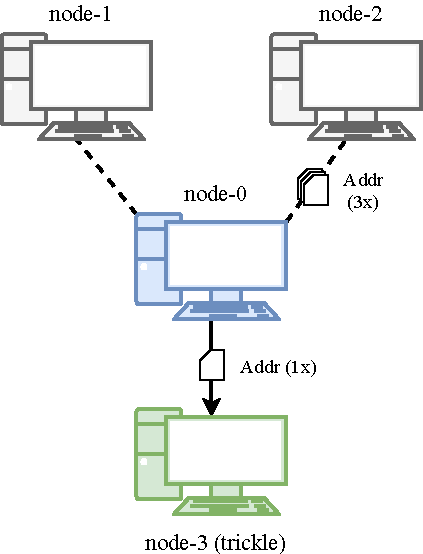
\includegraphics[width=\columnwidth]{figures/trickling_1}
		\vspace*{0.1cm}
		\caption{
			Round \num{1}:
			\texttt{node-3} is selected as trickle.
		}
		\vspace*{0.2cm}
	\end{subfigure}
	\hfill
	\begin{subfigure}{.4\textwidth}
		\vspace*{0.25cm}
		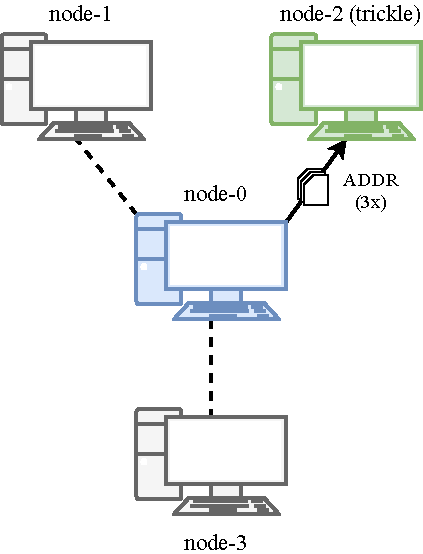
\includegraphics[width=\columnwidth]{figures/trickling_2}
		\vspace*{0.1cm}
		\caption{
			Round \num{2}:
			\texttt{node-2} is selected as trickle.
		}
		\vspace*{0.2cm}
	\end{subfigure}
	\caption[Illustration of the trickling procedure]{
		Illustration of the trickling procedure of \texttt{ADDR} messages.
		\texttt{node-0} (in blue) gets an \texttt{ADDR} message and select \texttt{node-3} and \texttt{node-2} for forwarding.
		An \texttt{ADDR} message is added to the queues of both nodes, that count respectively \num{1} and \num{3} messages.
		\texttt{node-3} is chosen at round \num{1} and its queue is flushed:
		the scheduled \texttt{ADDR} message is sent.
		\texttt{node-2} is chosen at round \num{2}:
		all \num{3} messages in queue are sent together to the destination.
	}
	\label{fig:trickling}
\end{figure}

\subsection{Peers cleanup}
Bitcoin nodes exchange control messages to verify that remote peers are still connected and working correctly.
Every \num{2} minutes, each node sends a \texttt{PING} message to all connected peers \cite{bitcoin_ping_pong}:
upon receiving a \texttt{PING} message, the node immediately replies with a \texttt{PONG}.
If a node does not receive any \texttt{PONG} message from a peer for \num{20} minutes, it assumes the peer to be not working and drops the connection.

\subsection{Messages}
TODO

\subsubsection{VERSION}
\label{par:version}
TODO

\subsubsection{VERACK}
TODO

\subsubsection{GETADDR}
TODO

\subsubsection{ADDR}
TODO

\subsubsection{PING}
TODO

\subsubsection{PONG}
TODO


\section{Core}
The core layer uses the underlying overlay network created by the topology layer to propagate blocks and transactions to all Bitcoin nodes.

\subsection{Messages}
TODO
